\section{Theorie}
\label{sec:Theorie}
Durch verschiedene experimentelle Befunde kann Licht nur durch die Quantenelektrodynamik widerspruchsfrei beschrieben werden. 
Für eine große Anzahl an Photenen kann Licht dabei als Welle genähert werden, wie es zum Beispiel in der Beugungsoptik geschieht. 
Wechselwirkt das Licht jedoch mit Materie, wie es bei dem Photoeffekt der Fall ist, können die auftretenden Phänomene mit dem 
Korpuskelmodell erklärt werden, in welcher die Quantelung des Lichts in einzelne Photonen angenommen wird. Im Folgenden soll 
das Licht dabei nach dem Korpuskelmodell behandelt werden. 

\subsection{Die Phänomene und Erklärung des Photoeffekts}
\label{sec:phänomene}
Wird eine Metalloberfläche mit Photenen der Energie 
\begin{equation}
    E_{P}=h\nu
    \label{eqn:photon}
\end{equation}
bestrahlt, können durch diese Elektronen aus dem Metall herrausgelöst werden. Dabei überträgt das Photon seine Energie dem im Metall 
befindelichen Elektron. %, welches schon eine kinetische Energie $E_{kin}\geq 0$ besitzt. 
%Was ist hier mit der Anfangsenergie?
Zum Verlassen des Metalls muss die spezifische 
Austrittsarbeit $\Phi_K$ geleistet werden. Die restliche Energie wird in kinetische Energie $E_{kin}\geq 0$ des Elektrons umgesetzt. Die 
Energiebilanz lautet demnach
\begin{equation}
    h\nu=\Phi_K+E_{kin}\;.
    %h\nu+E_{kin}=\Phi_K+E'_{kin}\;.
    \label{eqn:bilanz}
\end{equation}
Die Energie $E_{kin}$ der Elektronen nach dem Stoß ist also proportional zur Frequenz $\nu$ des Lichts.
Offensichtlich kann der Photoeffekt nur auftreten, wenn
\begin{equation*}
    h\nu<\Phi_K
\end{equation*}
gilt. Es existiert also eine minimale Grenzfrequenz unterhalb derer der Photoeffekt nicht auftritt.
Desweiteren ist zu beobachten, dass die Anzahl der ausgelösten Elektronen proportional zur Intensität des Lichtes ist. 

\subsection{Experimenteller Nachweis des Photoeffekts}
\label{sec:nachweis}
Für den Nachweis des Photoeffekts müssen die ausgelösten Elektronen gemessen werden. Dies geschieht durch eine positiv gelandene 
Auffängeranode, die sich gegenüber der Photokahode befindet. Trifft nun ein Elektron auf die Auffängeranode, wird ein Strom
gemessen. In Abbildung \ref{fig:Anordnung1} ist dieses Prinzip noch einmal veranschaulicht. In Abbildung \ref{fig:Photozelle} ist 
die verwendete Photozelle skizziert, in welcher sich sowohl Anode als auch Kathode befinden. Die Kathode besteht dabei aus einer dünnen
Metallschicht im Inneren der Photozelle. Die Anode ist durch einen Drahtring wenige Millimeter vor der Kathode realisiert. Das Innere des
Glaskolbens, in welchem sich die Elektroden befinden, ist weitestgehend evakuiert um Störeffekte mit Gasmolekülen zu vermeiden. 

\begin{figure}
    \centering
    \begin{subfigure}[b]{0.45\linewidth}
        \centering
        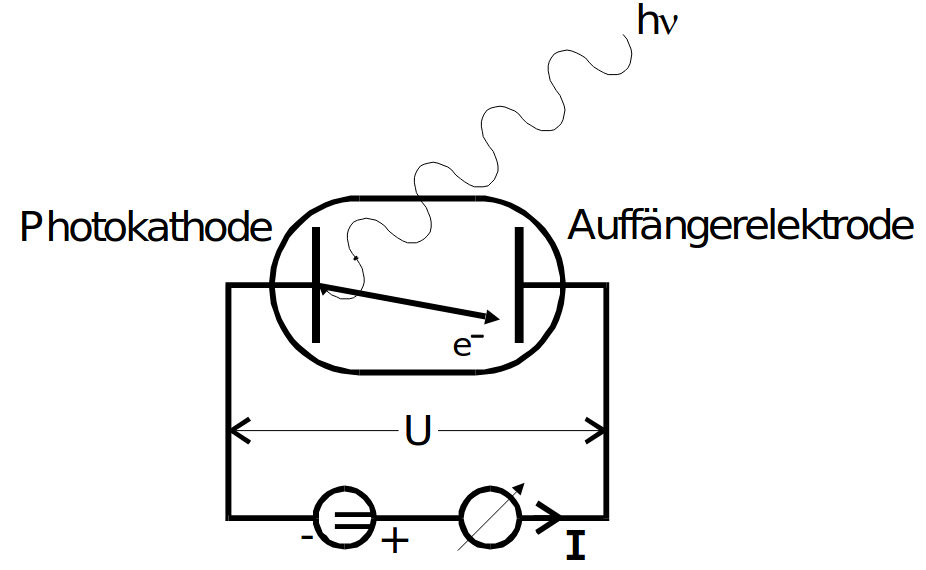
\includegraphics[width=\textwidth]{pictures/Anordnung1.png}
        \caption{Schematischer Versuchsaufbau. \cite{AP01}}
        \label{fig:Anordnung1}
    \end{subfigure}
    \hspace{.1\linewidth}% Abstand zwischen Bilder
    \begin{subfigure}[b]{0.3\linewidth}
        \centering
        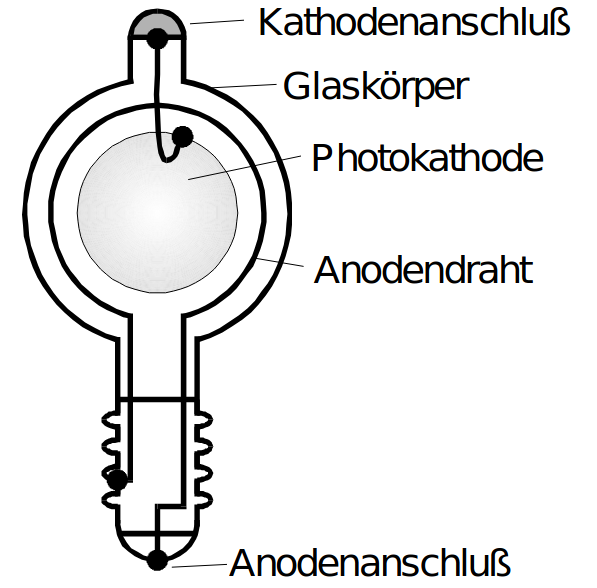
\includegraphics[width=\textwidth]{pictures/Photozelle.png}
        \caption{Skizze der Photozelle. \cite{AP01}}
        \label{fig:Photozelle}
    \end{subfigure}
\end{figure}

\noindent
Zwischen Kathode und Anode wird ein elektrisches Bremsfeld erzeugt, indem eine variable Spannungsquelle angeschlossen wird. Zur Messung der 
ausgelösten Elektronen wird ein Picoampermeter verwenendet. Die elektrische Schaltung ist in Abbildung \ref{fig:Schaltung} dargestellt. 
\begin{figure}
    \centering
    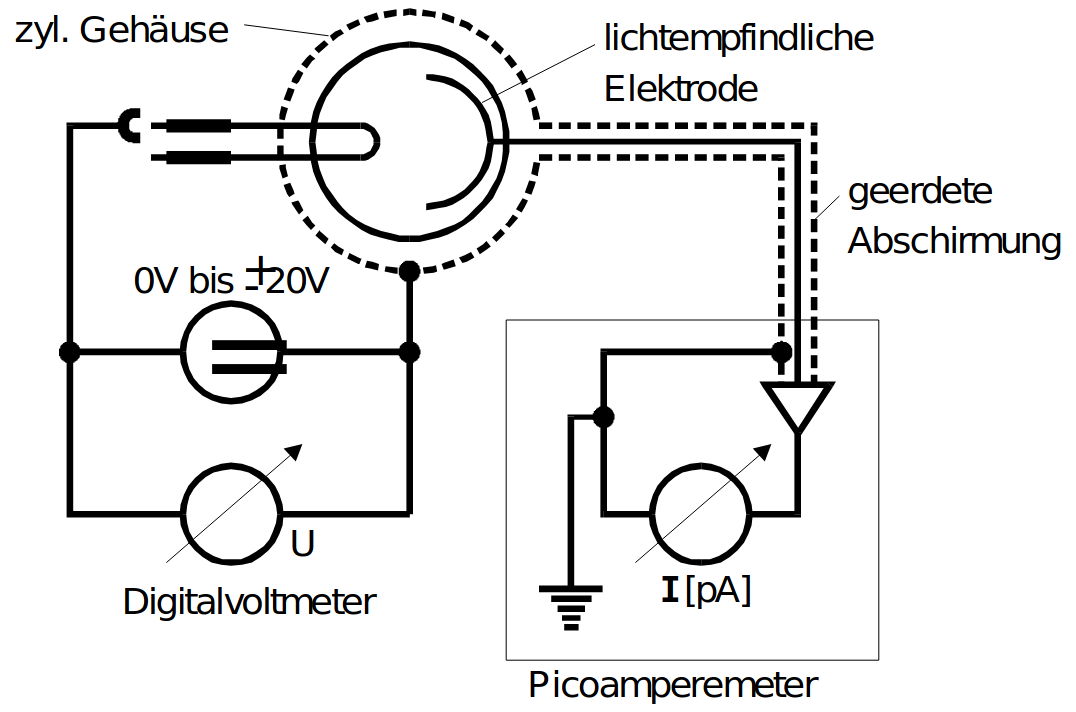
\includegraphics[scale=0.3]{pictures/ElektischeSchaltung.png}
    \caption{Elektrisches Schaltbild der Apperatur. \cite{AP01}}
    \label{fig:Schaltung}
\end{figure}

\noindent
Durch das Bremsfeld mit der Spannung $U_B$ können nur die Elektronen die Auffängeranode erreichen, deren Energie $E_{kin}>e_0U_B$ erfüllt.
Für die Grenzspannung 
\begin{equation}
    e_0=\frac{1}{2}m_0v_{max}^2 
\end{equation}
verschwindet der gemessene Strom, da selbst die Energie der schnellsten Elektronen nicht ausreicht um die Anode zu erreichen. Nach 
Gleichung \eqref{eqn:bilanz} gilt für diese Elektronen 
\begin{equation}
    h\nu=\Phi_K+e_0U_g\;.
\end{equation}
Die Elektronen, die eine Geschwindigkeit $v<v_{max}$ besitzen, erreichen schon für eine Spannung $U_B<U_g$ nicht mehr die Anode. Deswegen 
sinkt der gemessene Photostrom kontinuierlich ab, bis er bei $U_g$ null erreicht. Dies ist in Abbildung \ref{fig:Photostrom} in einem 
($U_B$-$I_P$)-Diagramm dargestellt. 

\begin{figure}
    \centering
    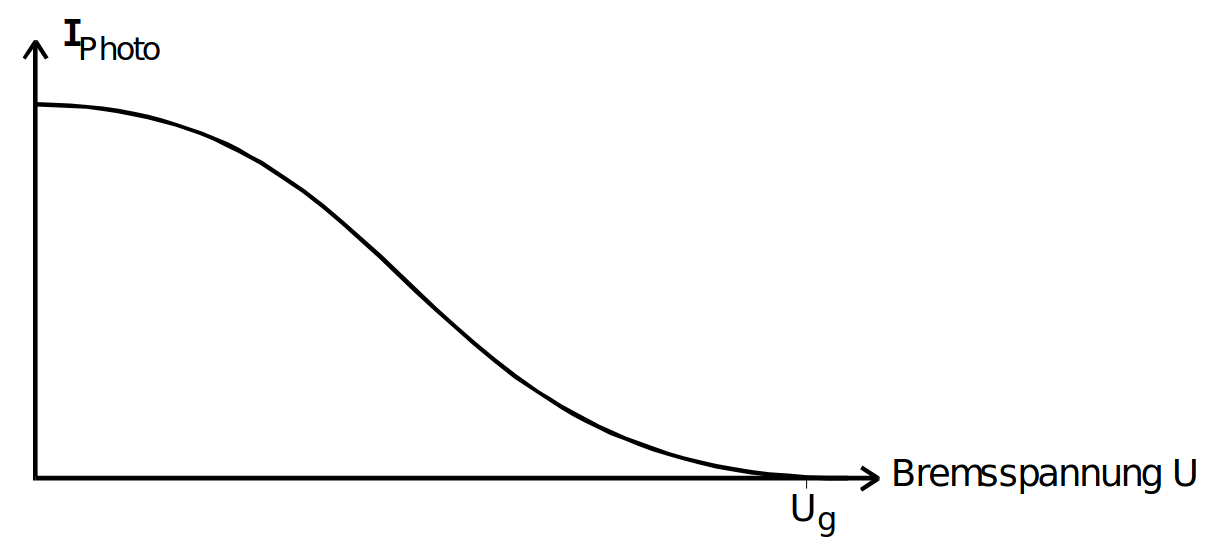
\includegraphics[scale=0.3]{pictures/Photostrom.png}
    \caption{Photostrom $I_{P}$ in Abhängigkeit der Bremsspannung $U_B$. \cite{AP01}}
    \label{fig:Schaltung}
\end{figure}

\noindent
Die unterschiedlichen Geschwindigkeiten der ausgelösten Elektronen resultiert aus der bereits im Metall vorhandenen kinetischen Energie der 
Elektronen, welche einer Fermi-Dirac-Verteilung folgt. 
\\\noindent
Unter bestimmten Vorraussetzungen lässt sich zwischen dem gemessenen Strom $I_{P}$ und der Bremsspannung $U_B$ der Zusammenhang 
\begin{equation*}
    I_{P}\propto U^2_g
\end{equation*}
zeigen. 
\\\noindent
Für den Fall, dass zwar $\Phi_K<h\nu$ gilt, also Elektronen aus der Kathode gelöst werden, aber für die Austrittsarbeit der Anode 
$\Phi_A>h\nu$ gilt, wird kein Strom auf der Anode gemessen, da die Elektronen durch das Gegenfeld zu stark abgebremst werden.
%Welches Gegenfeld bitte???
Mit einem beschleunigenden Potential $U_b$ kann jedoch wieder ein Strom gemessen werden, sobald 
\begin{equation*}
    h\nu+e_0U_{b}\geq \Phi_A
\end{equation*}
gilt.